\documentclass[a4paper, 12pt]{article}
\newcommand{\template}{../../Templates}
\usepackage{\template/package}
\usepackage{longtable}
\usepackage{enumitem}

\graphicspath{{../../Assets}}

\newcommand{\Descrizione}{Documento contenente le informazioni relative al controllo qualità}
\newcommand{\Titolo}{Piano di qualifica}
\newcommand{\Data}{20/11/2023}
\newcommand{\Versione}{0.1.0}
\newcommand{\Stato}{Non approvato}
\newcommand{\Verificatori}{Nessuno}
\newcommand{\Destinatari}{prof. Tullio Vardanega \\ & prof. Riccardo Cardin}

\newcommand{\Gruppo}{SWEnergy}
\newcommand{\Mail}{\href{mailto:project.swenergy@gmail.com}{project.swenergy@gmail.com}}

\renewcommand\familydefault{\sfdefault} % Set default font family to sans-serif
\linespread{1.5}

\hypersetup{
	pdfmenubar=true,            % show Acrobat’s menu?
	pdfstartview={FitH},        % fits the width of the page to the window
	colorlinks=true,            % false: boxed links; true: colored links
	linkcolor=black,            % color of internal links (change box color with linkbordercolor)
	% citecolor=green,          % color of links to bibliography
	% filecolor=magenta,        % color of file links
	urlcolor=[RGB]{156,1,198}   % color of external links
}

\newcommand{\copertina}{
	\begin{titlepage}
		\vspace*{-3.5cm}
		\makebox[\textwidth]{
\includegraphics[width=\paperwidth]{header.png}}
		\begin{center}
			
\includegraphics[width=1\textwidth]{logo.png}	\\
			\vspace{1cm}
			\Mail	\\
			\vspace{0.5cm}
			\textbf{\begin{LARGE} \Titolo \end{LARGE}}		\\
			\vspace{1cm}
			\textbf{Descrizione:} \Descrizione{}			\\
			\vspace{1cm}
			\begin{tabular}{ll}
				\textbf{Stato}               & \Stato              \\
				\textbf{Data}                & \Data               \\
				\midrule
				\textbf{Redattori}           & \Redattori          \\
				\textbf{Verificatori}        & \Verificatori       \\

				\ifdefined\Approvatori
				\textbf{Approvatori}         & \Approvatori        \\
				\fi

				\ifdefined\ApprovatoriInterni
				\textbf{Approvatori interni} & \ApprovatoriInterni \\
				\fi

				\ifdefined\ApprovatoriEsterni
				\textbf{Approvatori esterni} & \ApprovatoriEsterni \\
				\fi

				\ifdefined\Destinatari
				\textbf{Destinatari}         & \Destinatari        \\
				\fi

				\midrule

				\ifdefined\Versione
				\textbf{Versione}            & \Versione           \\
				\fi
			\end{tabular}
		\end{center}
		\vspace{4cm}
	\end{titlepage}
	\newpage
}

\fancypagestyle{plain}{
	\fancyhf{}
	\rhead{ 
\includegraphics[scale=0.05]{horizontal_logo.png}}
	\lhead{\Titolo \ifdefined\Versione \ \Versione \fi}
	%\lfoot{\Titolo}
	\rfoot{\thepage{} di \pageref{LastPage}}
	\renewcommand{\headrulewidth}{0.2pt}
	\renewcommand{\footrulewidth}{0.2pt}
}
\pagestyle{plain}


\begin{document}
\copertina{}
\section*{Registro delle modifiche}
 {
  \scriptsize
  \begin{tabular}{p{0.10\linewidth}p{0.10\linewidth}p{0.15\linewidth}p{0.15\linewidth}p{0.15\linewidth}p{0.19\linewidth}}
	  \textbf{Versione} & \textbf{Data} & \textbf{Redattore}     & \textbf{Verificatore} & \textbf{Approvatore} & \textbf{Descrizione}                                                                                                                     \\
	  \toprule
	  2.0.1             & 27/02/2024    & Davide Maffei          & Carlo Rosso           & /                    & Correzioni in seguito alla revisione RTB                                                                                                 \\
	  \hline
	  2.0.0             & 27/02/2024    & /                      & /                     & Niccolò Carlesso     & Approvazione finale del documento                                                                                                        \\
	  \hline
	  1.5.0             & 26/02/2024    & Alessandro Tigani Sava & Carlo Rosso           & /                    & Descrizione metriche di qualità                                                                                                          \\
	  \hline
	  1.4.1             & 14/02/2024    & Davide Maffei          & Giacomo Gualato       & /                    & Allineamento delle sezioni dei ruoli                                                                                                     \\
	  \hline
	  1.4.0             & 14/02/2024    & Davide Maffei          & Giacomo Gualato       & /                    & Creazione delle sezioni dei processi primari, di supporto e organizzativi                                                                \\
	  \hline
	  1.3.0             & 8/01/2024     & Carlo Rosso            & Niccolò Carlesso      & /                    & Correzione della sotto-sezione "Aggiornamento delle "Norme di Progetto"" e aggiunte le sotto-sezioni "Revisione del codice" e "Codifica" \\
	  \hline
	  1.2.0             & 31/12/2023    & Carlo Rosso            & Niccolò Carlesso      & /                    & Ristrutturazione del documento per ruolo, piuttosto che per argomento                                                                    \\
	  \hline
	  1.1.0             & 30/10/2023    & Carlo Rosso            & Giacomo Gualato       & /                    & Aggiornamento della sezione dedicata alla documentazione e aggiunta una sezione dedicata agli appunti                                    \\
	  \hline
	  1.0.0             & 30/10/2023    & /                      & /                     & Giacomo Gualato      & Approvazione finale del documento                                                                                                        \\
	  \hline
	  0.2.1             & 29/10/2023    & Alessandro Tigani Sava & Niccolò Carlesso      & /                    & Modifica procedure in sezione Approvazione di un documento                                                                               \\
	  \hline
	  0.2.0             & 24/10/2023    & Matteo Bando           & Niccolò Carlesso      & /                    & Redazione sezioni Versionamento, Verifica di un documento, Approvazione di un documento                                                  \\
	  \hline
	  0.1.0             & 23/10/2023    & Alessandro Tigani Sava & Matteo Bando          & /                    & Redazione sezioni Introduzione, Strumenti, Creazione e modifica di un documento, Ruoli, Registro delle modifiche                         \\
	  \hline
  \end{tabular}
 }


\tableofcontents
\newpage

\section{Introduzione}

Il presente documento, intitolato "Piano di Progetto", descrive e spiegare le
decisioni organizzative adottate dal gruppo SWEnergy per lo sviluppo del
progetto "\textit{Easy Meal}", proposto dall'azienda
\href{https://imolainformatica.it/}{Imola Informatica}. Il "Piano di Progetto" è
suddiviso nelle seguenti sezioni:

\begin{itemize}
	\item \textbf{Analisi dei rischi}: identifica i rischi individuati dal
	      gruppo e le strategie per mitigarli;

	\item \textbf{Modello di sviluppo}: descrive l'organizzazione temporale del
	      team di SWEnergy;

	\item \textbf{Pianificazione}: dettaglia la pianificazione del lavoro del
	      gruppo, incluse le attività, le risorse e i tempi necessari per lo
	      sviluppo del progetto;

	\item \textbf{Preventivo}: presenta il preventivo delle ore di lavoro e il
	      costo totale del progetto;

	\item \textbf{Consuntivo}: riporta le ore di lavoro e il costo effettivo del
	      progetto fino al momento della stesura del piano di progetto della
	      fase corrente: RTB.
\end{itemize}

\subsection{Scopo del documento}

Questo documento ha lo scopo di raccogliere in modo organico, coerente e
uniforme tutte le informazioni riguardanti la pianificazione del progetto, al
fine di fornire un riferimento per la gestione dello stesso. Al termine della
prima fase del progetto (RTB), verrà utilizzato per valutare l'andamento del
lavoro e per spiegare le decisioni adottate durante la pianificazione.

\subsection{Scopo del prodotto}

"\textit{Easy Meal}" è una web app progettata per gestire le prenotazioni
presso i ristoranti, sia dal lato dei clienti che dei ristoratori. Il prodotto
finale sarà composto da due parti:

\begin{itemize}
	\item \textbf{Cliente}: consente ai clienti di prenotare un tavolo presso un
	      ristorante, visualizzare il menù e effettuare un ordine;

	\item \textbf{Ristoratore}: consente ai ristoratori di gestire le
	      prenotazioni e gli ordini dei clienti, oltre a visualizzare la lista
	      degli ingredienti necessari per preparare i piatti ordinati.
\end{itemize}

\subsection{Glossario}

Al fine di evitare ambiguità linguistiche e garantire un'utilizzazione coerente
delle terminologie nei documenti, il gruppo ha redatto un documento interno
chiamato "Glossario". Questo documento definisce in modo chiaro e preciso i
termini che potrebbero generare ambiguità o incomprensione nel testo. I termini
presenti nel Glossario sono identificati da una 'G' (per esempio parola$_G$) a
pedice.

\subsection{Riferimenti}

\subsubsection{Normativi}
\begin{itemize}
	\item "\textit{Way of Working}";
	\item 	\href{https://www.math.unipd.it/~tullio/IS-1/2023/Progetto/C3.pdf}
	      {Documento del capitolato d'appalto C3 - \textit{Easy Meal}};
	\item \href{https://www.math.unipd.it/~tullio/IS-1/2023/Dispense/PD2.pdf}
	      {Regolamento del progetto};
\end{itemize}

\subsubsection{Informativi}

Slide dell'insegnamento di Ingegneria del Software:
\begin{itemize}
	\item \href{https://www.math.unipd.it/~tullio/IS-1/2023/Dispense/T3.pdf}
	      {Modelli di sviluppo del software};
	\item \href{https://www.math.unipd.it/~tullio/IS-1/2023/Dispense/T4.pdf}
	      {Gestione di progetto};
	\item \href{https://www.math.unipd.it/~tullio/IS-1/2023/Dispense/T5.pdf}
	      {Analisi dei requisiti};
\end{itemize}

\subsection{Scadenze}
Il \textit{team} di SWEnergy si impegna a rispettare le seguenti scadenze per il
completamento del progetto:
\begin{itemize}
	\item \textbf{Prima revisione (avanzamento RTB}: 21 dicembre 2023;
	\item \textbf{Seconda revisione (avanzamento PB)}: da definire;
	\item \textbf{Terza revisione (avanzamento CA)}: da definire;
\end{itemize}

\section{Qualità di processo}
\subsection{Introduzione}
La qualità del risultato finale è intrinsecamente legata all'efficienza e alla qualità dei processi coinvolti. 
Per garantire il rispetto degli standard di qualità definiti, diventa cruciale impiegare metriche di valutazione adeguate.\\
Nella presente sezione, vengono illustrati i valori accettabili e ottimali in termini di qualità, basati su metriche delineate nel documento "Norme di Progetto". \\
È di primaria importanza sorvegliare costantemente tali metriche al fine di assicurare che i processi corrispondano agli obiettivi di qualità prefissati e che, di conseguenza, il prodotto conclusivo risulti di elevata qualità.\\

\noindent
Questo standard categorizza i processi in tre macroaree principali:
\begin{itemize}
    \item Processi primari.
    \item Processi organizzativi.
    \item Processi di supporto.
\end{itemize}


\subsection{Processi primari}
Si sudddividono in:
\begin{itemize}
    \item \textbf{Fornitura}: finalizzata all'identificazione di procedure e risorse atte a soddisfare i requisiti di progetto.
    \item \textbf{Sviluppo}: inerente alle attività per la realizzazione del prodotto.
\end{itemize}

\subsubsection{Valori di riferimento}
Si utilizzano i seguenti acronimi per indicare le metriche:
\begin{itemize}
    \item \textbf{BAC}: \textit{Budget at Completion}, il preventivo presentato al proponente.
\end{itemize}

\begin{table}[H]
    \centering
    \begin{tabularx}{\textwidth}{p{3.5cm}|X|X|l|l}
        \hline
        \multicolumn{2}{l|}{\textbf{Metrica}} & \textbf{Codice}   & \textbf{Valore ottimale}  & \textbf{Valore accettabile}   \\
        \hline
        \multicolumn{5}{c}{\textbf{Fornitura}} \\
        \hline
        Schedule Variance               & SV    & MPC01 & 0\%               & $\ge -10\%$                   \\
        Budget Variance                 & BV    & MPC02 & 0\%               & $\ge -10\%$                   \\
        Estimated at Completion         & EAC   & MPC03 & EAC = BAC         & $\text{EAC} \in (\text{BAC} \pm 5\%)$  \\
        Budgeted Cost of Work Scheduled & BCWS  & MPC04 & $\le$ BAC         & $\ge 0$                       \\
        Budgeted Cost of Work Performed & BCWP  & MPC05 & BCWP = BCWS       & $\le$ BCWS $+ 5\%$            \\
        Actual Cost of Work Performed   & ACWP  & MPC06 & $\le$ BCWS   & BCWS $+ 5\%$                       \\
        \hline
        \multicolumn{5}{c}{\textbf{Sviluppo}} \\
        \hline 
        Requirements stability index    & RSI   & MPC07 & 100\%             & $ge$ 80\%                     \\
        Satisfied obligatory requirements & SOR & MPC08 & 100\%             & 100\%                         \\
        \hline
    \end{tabularx}
    \caption{Valori di riferimento per le metriche dei processi primari}
\end{table}


\subsection{Processi organizzativi}
\subsubsection{Valori di riferimento}
\subsection{Processi di supporto}
\subsubsection{Valori di riferimento}

\section{Qualità di prodotto}
La qualità di prodotto viene garantita dall'adozione dello standard \textbf{ISO/IEC 9126} che propone caratteristiche di qualità misurabili attraverso metriche ben definite.

\subsection{Obiettivi}
Si effettua una suddivisione in:
\begin{itemize}
    \item \textbf{Qualità interna}: fa riferimento alla qualità della documentazione interna prodotta.
    \item \textbf{Qualità esterna}: fa riferimento alla qualità del software rilasciato.
\end{itemize}

\subsubsection{Qualità interna}
Volge al raggiungimento dei seguenti obiettivi:
\begin{itemize}
    \item \textbf{Usabilità}: comprensibilità e leggibilità della documentazione prodotta.
\end{itemize}
\begin{table}[H]
    \centering
    \begin{tabularx}{\textwidth}{p{3.5cm}|X|l|l}
        \hline
        \textbf{Metrica} & \textbf{Codice}   & \textbf{Valore ottimale}  & \textbf{Valore accettabile}   \\
        \hline
        \multicolumn{4}{c}{\textbf{Usabilità}} \\
        \hline
        Indice di Gulpease & MPD1 &  $\ge 90\%$ & $\ge 70\%$    \\
        \hline
    \end{tabularx}
    \caption{Valori di riferimento per le metriche di qualità interna}
\end{table}

\subsubsection{Qualità esterna}
Volge al raggiungimento dei seguenti obiettivi:
\begin{itemize}
    \item \textbf{Funzionalità}: il prodotto deve soddisfare i requisiti stabiliti in fase di analisi.
    \item \textbf{Affidabilità}: sotto determinate condizioni il prodotto deve mantenere un determinato livello di prestazioni per un periodo di tempo prestabilito.
    \item \textbf{Efficienza}: il prodotto deve raggiungere l'obiettivo minimizzando l'utilizzo delle risorse .
    \item \textbf{Usabilità}: l'utente deve essere in grado di utilizzare il prodotto e comprenderne le sue funzioni.
    \item \textbf{Manutenibilità}: il prodotto deve poter essere modificato nel tempo senza che gli aggiornamenti ne compromettano le funzionalità.
    \item \textbf{Portabilità}: il prodotto deve essere fruibile in ambienti diversi
\end{itemize}
\begin{table}[H]
    \centering
    \begin{tabularx}{\textwidth}{p{5.5cm}|X|l|l}
        \hline
        \textbf{Metrica} & \textbf{Codice}   & \textbf{Valore ottimale}  & \textbf{Valore accettabile}   \\
        \hline
        \multicolumn{4}{c}{\textbf{Funzionalità}} \\
        \hline
        Copertura dei requisiti & MPD2 &  $100\%$ & $100\%$    \\
        \hline
        \multicolumn{4}{c}{\textbf{Affidabilità}} \\
        \hline
        Densità di failure & MPD3 & $\le 10\%$ & $\le 20\% $ \\
        \hline
        \multicolumn{4}{c}{\textbf{Efficienza}} \\
        \hline
        Tempo medio di risposta & MPD4 & 2 secondi & 3 secondi \\
        \hline
        \multicolumn{4}{c}{\textbf{Usabilità}} \\
        \hline
        Average cyclomatic complexity & MPD5 & 10 & 20 \\
        Facilità di utilizzo & MPD6 & 5 click & $\le 10$ click \\
        Facilità di apprendimento delle funzionalità & MPD7 & $\le 5$ minuti & $\le 15$ minuti \\
        \hline
        \multicolumn{4}{c}{\textbf{Manutenibilità}} \\
        \hline
        Comprensibilità del codice & MPD8 & $\ge 80\%$ & $\ge 70\%$ \\
        \hline
        \multicolumn{4}{c}{\textbf{Portabilità}} \\
        \hline
        Browser supportati & MPD9 & $100\%$ & $\ge 80\%$ \\
        \hline
    \end{tabularx}
    \caption{Valori di riferimento per le metriche di qualità esterna}
\end{table}
\section{Test}
La verifica del prodotto necessita l'esecuzione di test mirati, questi verranno eseguiti contemporaneamente allo sviluppo per garantire la correttezza del software in ogni momento.
Le tipologie di test previste sono:
\begin{itemize}
    \item \textbf{Test di unità}: utilizzati per valutare le singole componenti del sistema come classi e metodi, non considerano le dipendenze tra le classi (che sovranno esistere solo in caso gli elementi debbano essere testati insieme).
    Sono definiti durante la progettazione.
    \item \textbf{Test di integrazione}: verificano l'integrazione tra le componenti del sistema.
    \item \textbf{Test di sistema}: vengono effettuati basandosi su quanto emerso durante l'analisi dei requisiti per verificarne la corretta implementazione.
    \item \textbf{Test di accettazione}: utilizzati per verificare che il software soddisfi i requisiti presentati nel capitolato in modo da essere pronto per la consegna, svolti in presenza del committente.    
\end{itemize}

\subsection{Test di sistema}
La nomenclatura utilizzata per identificare i test è spiegata nel documento Norme di Progetto v2.0.0.

\setlist{nolistsep}
\fontsize{10}{12}\selectfont
\begin{longtable}{|p{0.12\linewidth}|p{0.58\linewidth}|p{0.22\linewidth}|}
    \hline
	\textbf{Codice} & \textbf{Descrizione} & \textbf{Stato} \\
    \hline
    TS.RFO1 & 
    L'Utente base e generico deve poter consultare l'elenco dei ristoranti disponibili. \par 
    Verificare che: 
    \begin{itemize}
        \item la \textit{Home} della piattaforma sia visualizzabile senza richiedere l'accesso.
        \item la \textit{Home} della piattaforma mostri l'elenco dei ristoranti disponibili.
        \item il pulsante per il ritorno alla \textit{Home} sia ben riconoscibile.
        \item sia possibile selezionare la città di interesse dalla \textit{Home}.
    \end{itemize}&
    Non implementato \\
    \hline
    TS.RFO2 & 
    L'Utente base e generico devono poter visualizzare in dettaglio un ristorante \par 
    Verificare che: 
    \begin{itemize}
        \item la \textit{Home} della piattaforma sia visualizzabile senza richiedere l'accesso.
        \item il dettaglio di un ristorante deve essere visualizzabile senza richiedere l'accesso.
        \item siano presenti ristoranti nell'elenco visualizzato dall'utente.
        \item la scheda del ristorante sia selezionabile.
    \end{itemize}&
    Non implementato \\
    \hline
    TS.RFO3 & 
    L'Utente base e generico devono poter condividere un link di un ristorante. \par 
    Verificare che: 
    \begin{itemize}
        \item la \textit{Home} della piattaforma sia visualizzabile senza richiedere l'accesso.
        \item il dettaglio di un ristorante deve essere visualizzabile senza richiedere l'accesso.
        \item la pagina di un ristorante deve essersi caricata correttamnte.
        \item il pulsante di condivisione deve essere individuabile.
    \end{itemize}&
    Non implementato \\
    \hline
    TS.RFO4 & 
    L'Utente base e generico devono poter visualizzare la pagina delle FAQ. \par 
    Verificare che: 
    \begin{itemize}
        \item il pulsante per la visualizzazione delle FAQ deve essere individuabile.
        \item la pagina di visualizzazione delle FAQ deve essere visitabile senza richiedere l'accesso.
    \end{itemize}&
    Non implementato \\
    \hline
    TS.RFO5 & 
    L'Utente generico e ristoratore devono poter comunicare tra loro attraverso chat \par 
    Verificare che: 
    \begin{itemize}
        \item TODO
    \end{itemize}&
    Non implementato \\
    \hline
    TS.RFO6 & 
    Il Sistema invia una notifica agli utenti collegati nella chat \par 
    Verificare che: 
    \begin{itemize}
        \item l'utente sia registrato nel sistema.
        \item l'utente a cui è destinata la notifica sia connesso al sistema.
    \end{itemize}&
    Non implementato \\
    \hline
    TS.RFO7 & 
    L'Utente generico effettua l'accesso al Sistema \par 
    Verificare che: 
    \begin{itemize}
        \item l'utente sia registrato nel sistema.
        \item l'utente non abbia già effettuato l'acesso al sistema.
        \item il pulsante per effettuare l'accesso sia ben visibile e chiaro.
        \item il pulsante per effettuare l'accesso rimandi alla pagina di inserimento credenziali.
    \end{itemize}&
    Non implementato \\
    \hline
    TS.RFO8 & 
    L'Utente generico effettua la registrazione al Sistema. \par 
    Verificare che: 
    \begin{itemize}
        \item l'utente non sia registrato nel sistema.
        \item l'utente non abbia già effettuato l'acesso al sistema.
        \item il pulsante per effettuare la registrazione sia ben visibile e chiaro.
        \item il pulsante per effettuare la registrazione rimandi alla pagina di inserimento dati.
    \end{itemize}&
    Non implementato \\
    \hline
    TS.RFD10 & 
    L'Utente base deve visualizzare e modificare i propri dati. \par 
    Verificare che: 
    \begin{itemize}
        \item l'utente deve essere correttamente autenticato.
        \item il pulsante per accedere alla gestione dei dati sia ben visibile e chiaro.
        \item il pulsante rimandi alla pagina di gestione dati.
        \item i nuovi dati inseriti non contengano caratteri non permessi dal sistema.
    \end{itemize}&
    Non implementato \\
    \hline
    TS.RFD12 & 
    L'Utente base deve visualizzare le proprie prenotazioni. \par 
    Verificare che: 
    \begin{itemize}
        \item l'utente deve essere correttamente autenticato.
        \item il pulsante per accedere alla visualizzazione delle prenotazioni sia ben visibile e chiaro.
        \item il pulsante rimandi correttamente alla pagina di visualizzazione delle prenotazioni.
    \end{itemize}&
    Non implementato \\
    \hline
    TS.RFD13 & 
    L'Utente base e ristoratore devono effettuare il \textit{logout}. \par 
    Verificare che: 
    \begin{itemize}
        \item l'utente deve essere correttamente autenticato.
        \item il pulsante per effettuare la disconnessione sia ben visibile e chiaro.
        \item il pulsante disconnetta correttamente l'utente e lo rimandi ala \textit{Home} della piattaforma.
    \end{itemize}&
    Non implementato \\
    \hline
    TS.RFD14 & 
    L’Utente base deve poter eliminare il suo account. \par 
    Verificare che: 
    \begin{itemize}
        \item l'utente deve essere correttamente autenticato.
        \item il pulsante per richiedere l'eliminazione dei propri dati sia ben visibile e chiaro.
        \item il pulsante avvii correttamente la procedura di eliminazione dati relativi allo specifico utente.
    \end{itemize}&
    Non implementato \\
    \hline
    TS.RFO16 & 
    L’Utente base deve poter prenotare un tavolo.  \par 
    Verificare che: 
    \begin{itemize}
        \item l'utente deve essere correttamente autenticato.
        \item un ristorante deve essere attualmente selezionato.
        \item i dati necessari alla prenotazione siano stati inseriti e siano corretti.
        \item il pulsante per richiedere la prenotazione sia ben visibile e chiaro.
        \item il pulsante invii correttamente la richiesta di prenotazione.
    \end{itemize}&
    Non implementato \\
    \hline
    TS.RFO17 & 
    Il Sistema notifica l’Utente ristoratore dell’avvenuta prenotazione.  \par 
    Verificare che: 
    \begin{itemize}
        \item il corretto utente ristoratore sia autenticato nel sistema.
        \item il pulsante per visualizzare le prenotazioni mostri un indicatore di notifica.
    \end{itemize}&
    Non implementato \\
    \hline
    TS.RFO18 & 
    L’Utente base deve poter condividere la prenotazione con i commensali.  \par 
    Verificare che: 
    \begin{itemize}
        \item l'utente base è correttamente autenticato nel sistema.
        \item l'utente base ha una prenotazione in corso che è stata accettata dal ristoratore.
        \item il pulsante per la condivisione sia ben visibile e chiaro.
        \item il pulsante per la condivisione salvi il riferimento alla prenotazione nelle note del dispositivo utilizzato dall'utente.
    \end{itemize}&
    Non implementato \\
    \hline
    TS.RFO19 & 
    L’Utente base deve poter annullare la prenotazione.  \par 
    Verificare che: 
    \begin{itemize}
        \item l'utente base sia correttamente autenticato nel sistema.
        \item l'utente base abbia una prenotazione in corso.
        \item il pulsante per l'annullamento sia ben visibile e chiaro.
        \item il pulsante per l'annullamento modifichi correttamente lo stato della prenotazione.
    \end{itemize}&
    Non implementato \\
    \hline
    TS.RFO20 & 
    L’Utente base deve poter accedere ad una prenotazione.  \par 
    Verificare che: 
    \begin{itemize}
        \item l'utente base sia correttamente autenticato nel sistema.
        \item il \textit{link} relativo alla condivisione di una prenotazione è corretto.
        \item la pagina relativa alla prenotazione viene visualizzata correttamente.
    \end{itemize}&
    Non implementato \\
    \hline
    TS.RFO21 & 
    L’Utente base deve poter fare un ordinazione collaborativa dei pasti e creare il suo ordine.  \par 
    Verificare che: 
    \begin{itemize}
        \item l'utente base sia correttamente autenticato nel sistema.
        \item l'utente base abbia una prenotazione in corso.
        \item le ordinazioni degli altri utenti vengano correttamente visualizzate.
        \item le pietanze scelte dall'utente vengano correttamente aggiunte all'ordine.
        \item il pulsante di conferma sia ben visibile e chiaro.
    \end{itemize}&
    Non implementato \\
    \hline
    TS.RFO22 & 
    L’Utente base deve poter annullare il proprio ordine.   \par 
    Verificare che: 
    \begin{itemize}
        \item l'utente base sia correttamente autenticato nel sistema.
        \item l'utente base abbia una prenotazione in corso.
        \item le pietanze ordinate siano 
    \end{itemize}&
    Non implementato \\
\end{longtable}

\section{Attività di verifica}
Si analizzano qui le metriche:
\begin{itemize}
    \item \hyperref[s:mpc02]{\textbf{MPC02}}\textbf{}: \textit{Budget Variance}.
    \item \hyperref[s:mpc04]{\textbf{MPC04}}\textbf{}: \textit{Budgeted Cost of Work Scheduled}.
    \item \hyperref[s:mpc06]{\textbf{MPC06}}\textbf{}: \textit{Actual Cost of Work Performed}.
    \item \hyperref[s:mpc07]{\textbf{MPC07}}\textbf{}: \textit{Requirements stability index}.
    \item \hyperref[s:mpc08]{\textbf{MPC08}}\textbf{}: \textit{Satisfied obligatory requirements}.
    \item \hyperref[s:mpc09]{\textbf{MPC09}}\textbf{}: \textit{Non-calculated risk}.
    \item \hyperref[s:mpc10]{\textbf{MPC10}}\textbf{}: \textit{Code Coverage}.
    \item \hyperref[s:mpc11]{\textbf{MPC11}}\textbf{}: \textit{Passed Test Cases Percentage}.
    \item \hyperref[s:mpd1]{\textbf{MPD1}}\textbf{}: Indice di Gulpease.
    \item \hyperref[s:mpd2]{\textbf{MPD2}}\textbf{}: Copertura dei requisiti.
    \item \hyperref[s:mpd9]{\textbf{MPD9}}\textbf{}: Browser supportati.

\end{itemize}
\newpage


\subsection{MPC02 - Budget Variance}
\label{s:mpc02}
La \textit{Budget Variance} confronta il costo effettivo del lavoro completato fino a un certo punto nel tempo con il costo pianificato per quel lavoro.
Il valore negativo riportato in Figura \ref{fig:mpc02} indica che il costo effettivo è superiore al \textit{budget} pianificato.
Il valore medio riportato rientra nel margine di accettabilità stabilito. \\
Il gruppo ritiene che, nella prima fase RTB, lo sforamento del \textit{budget} sia dovuto alla generale inesperienza dei vari membri nella gestione di un progetto e nell'uso delle tecnologie, che ha portato alla necessità di incrementare il tempo di lavoro.\\
Nella seconda fase il gruppo ha individuato delle problematiche che non erano note nella fase precedente, questo grazie all'esperienza maturata durante lo sviluppo.
Tali problematiche hanno aumentato le attività da svolgere per mettere in atto operazioni di correzione, questo ha portato ad uno sforamento del \textit{budget}.
In particolare durante il sesto \textit{sprint}, il gruppo si è reso conto di aver sottostimato le ore necessarie per svolgere le attività di programmazione.
La pianificazione delle attività negli \textit{sprint} successivi è stata quindi rivista adeguando le ore necessarie alla programmazione con quandto sperimentato nello \textit{sprint} numero 6.

\begin{figure}[ht]
    \centering
    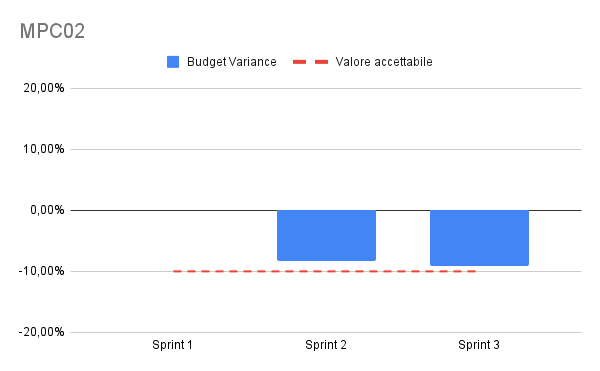
\includegraphics[width=0.8\textwidth]{img/MPC02.png}
    \caption{MPC02 - Budget Variance}
    \label{fig:mpc02}
\end{figure}

\newpage


\subsection{MPC04 - Budgeted Cost of Work Scheduled}
\label{s:mpc04}
Rappresenta il costo del lavoro pianificato per essere completato entro una data specifica nel progetto.\\
Nel grafico in Figura \ref{fig:mpc04} è stato inserito anche il costo relativo ad ogni \textit{sprint} al fine di indicare più intuitivamente il contributo di ogni singola fase al costo complessivo.\\
Il minor costo associato al quarto \textit{sprint} deriva dalla necessità di ridurre le ore di lavoro utile in concomitanza dei numerosi impegni, sia personali che legati alla sessione di esami, dei membri del gruppo.\\
Il consumo di risorse, confrontato con il preventivo dei costi presente nel documento \href{https://project-swenergy.github.io/Candidatura/Presentazione%20costi%20e%20assunzione%20impegni.pdf}{Presentazione costi ed assunzione impegni v2.0.0}, risulta ragionevole in considerazione della diversa durata delle fasi RTB e PB.\\
A partire dalla fase PB, relativa allo \textit{sprint} numero 5, si ha una crescita lineare costante che indica:
\begin{itemize}
    \item \textbf{Stima accurata}: le stime iniziali per il progetto sono precise e il lavoro si sta svolgendo secondo la pianificazione senza grandi variazioni o imprevisti.
    \item \textbf{Stabilità del processo}: indica che il processo utilizzato per completare il lavoro è stabile e prevedibile.
    \item \textbf{Controllo del progetto}: indica che il progetto è ben gestito e che ci sono processi di controllo efficaci per monitorare il progresso e intervenire tempestivamente in caso di deviazioni dalla pianificazione.
\end{itemize}
\vspace{1.5em}
Le problematiche riscontrate durante lo sviluppo sono quindi state correttamente gestite per consentire un progresso lineare e, quindi, più facilmente gestibile.
\begin{figure}[h]
    \centering
    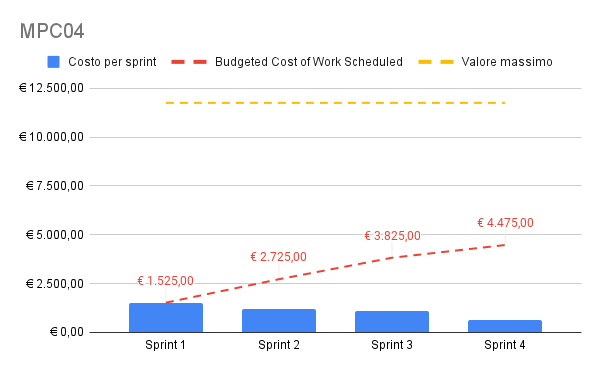
\includegraphics[width=0.8\textwidth]{img/MPC04.png}
    \caption{MPC04 - Budgeted Cost of Work Scheduled}
    \label{fig:mpc04}
\end{figure}


\subsection{MPC06 - Actual Cost of Work Performed}
\label{s:mpc06}
Il valore riportato in Figura \ref{fig:mpc06} indica che, a seguito del primo \textit{sprint}, il costo effettivo sostenuto ha superato quello preventivato.\\
Il gruppo ritiene che che il superamento del costo preventivato sia dovuto alla generale inesperienza dei vari membri nella gestione di un progetto e nell'uso delle tecnologie, che ha portato alla necessità di incrementare il tempo di lavoro nella fase iniziale del progetto.\\
Nonostante il superamento del valore ottimale, il costo effettivo è rimasto complessivamente all'interno del margine di accettabilità indicato nella metrica in esame.

\begin{figure}[htbp]
    \centering
    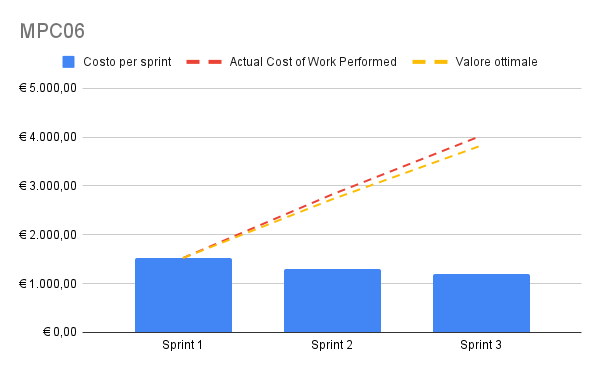
\includegraphics[width=0.7\textwidth]{img/MPC06.png}
    \caption{MPC06 - Actual Cost of Work Performed}
    \label{fig:mpc06}
\end{figure}


\subsection{MPC07 - Requirements stability index}
\label{s:mpc07}
Indica la stabilità dei requisiti nel corso del tempo.
Un RSI più alto indica una maggiore instabilità dei requisiti, mentre un RSI più basso indica una maggiore stabilità.
I requisiti sono stati aggiornati in seguito alla fase RTB, a seguito del dialogo con il proponente e alla presentazione del lavoro svolto.
Le modifiche apportate ai requisiti rientrano comunque all'interno del margine di accettabilità previsto.
\begin{table}[H]
    \centering
    \begin{tabularx}{\textwidth}{X|l|l|l|l}
        \hline
        \textbf{Metrica}             & \textbf{Codice} & \textbf{Valore ottimale} & \textbf{Valore accettabile} & \textbf{Valore attuale} \\
        \hline
        Requirements stability index & MPC07           & 0\%                      & 10\%                        & 8\%                     \\
        \hline
    \end{tabularx}
\end{table}


\subsection{MPC08 - Satisfied obligatory requirements}
\label{s:mpc08}
Il numero di requisiti obbligatori è stato ridotto a seguito del colloquio avuto con il proponente nell'ottavo \textit{sprint}.
La necessità di ridurre il numero di requisiti obbligatori è stata causata dal ritardo accumulato nello sviluppo e dalla necessità di mantenere il più possibile invariata la data di consegna del progetto.
Al termine del nono \textit{sprint} sono stati soddisfatti tutti i requisiti obbligatori individuati.
\begin{table}[H]
    \centering
    \begin{tabularx}{\textwidth}{X|l|l|l|l}
        \hline
        \textbf{Metrica}                  & \textbf{Codice} & \textbf{Valore ottimale} & \textbf{Valore accettabile} & \textbf{Valore attuale} \\
        \hline
        Satisfied obligatory requirements & MPC08           & 100\%                    & 100\%                       & 100\%                   \\
        \hline
    \end{tabularx}
\end{table}


\subsection{MPC09 - Non-calculated risk}
\label{s:mpc09}
Questa metrica si riferisce ai rischi che non sono stati attentamente valutati o considerati durante lo sviluppo del software.
Durante lo sviluppo del progetto i rischi sono stati valutati correttamente e sono state previste procedure per la mitigazione.
Le informazioni inerenti i rischi individuati dal gruppo sono visibili nel documento "Piano di Progetto v2.0.0".
\begin{table}[H]
    \centering
    \begin{tabularx}{\textwidth}{X|l|l|l|l}
        \hline
        \textbf{Metrica}    & \textbf{Codice} & \textbf{Valore ottimale} & \textbf{Valore accettabile} & \textbf{Valore attuale} \\
        \hline
        Non-calculated risk & MPC09           & 0                        & 5                           & 0                       \\
        \hline
    \end{tabularx}
\end{table}


\subsection{MPC10 - Code Coverage}
\label{s:mpc10}
Sono state valutate quattro misure inerenti la copertura del codice tramite test di unità.
Vengono qui riportate divise tra il gruppo dedicatosi al \textit{frontend} e quello dedicatosi al \textit{backend}.
Insieme alla metrica MPC11 fornisce una panoramica della qualità del codice.
\begin{table}[H]
    \centering
    \begin{tabularx}{\textwidth}{X|l|l|l|l}
        \hline
        \textbf{Metrica}    & \textbf{Codice} & \textbf{Valore ottimale} & \textbf{Valore accettabile} & \textbf{Valore attuale} \\
        \hline
        \textit{Statements} & MPC10           & $100\%$                  & $\ge 80\%$                  & $ 92\%$                 \\
        \hline
        \textit{Branches}   & MPC10           & $100\%$                  & $\ge 80\%$                  & $ 86\%$                 \\
        \hline
        \textit{Functions}  & MPC10           & $100\%$                  & $\ge 80\%$                  & $ 93\%$                 \\
        \hline
        \textit{Lines}      & MPC10           & $100\%$                  & $\ge 80\%$                  & $ 92\%$                 \\
        \hline
    \end{tabularx}
    \caption{\textit{Code coverage Frontend}}
\end{table}
\begin{table}[H]
    \centering
    \begin{tabularx}{\textwidth}{X|l|l|l|l}
        \hline
        \textbf{Metrica}    & \textbf{Codice} & \textbf{Valore ottimale} & \textbf{Valore accettabile} & \textbf{Valore attuale} \\
        \hline
        \textit{Statements} & MPC10           & $100\%$                  & $\ge 80\%$                  & $ 90\%$                 \\
        \hline
        \textit{Branches}   & MPC10           & $100\%$                  & $\ge 80\%$                  & $ 87\%$                 \\
        \hline
        \textit{Functions}  & MPC10           & $100\%$                  & $\ge 80\%$                  & $ 93\%$                 \\
        \hline
        \textit{Lines}      & MPC10           & $100\%$                  & $\ge 80\%$                  & $ 89\%$                 \\
        \hline
    \end{tabularx}
    \caption{\textit{Code coverage Backend}}
\end{table}


\subsection{MPC11 - Passed Test Cases Percentage}
Questo valore indica quanto sia riuscito il processo di testing rispetto al numero totale di casi di test eseguiti.
Insieme alla metrica MPC10 fornisce una panoramica della qualità del codice.

\label{s:mpc11}
\begin{table}[H]
    \centering
    \begin{tabularx}{\textwidth}{X|l|l|l|l}
        \hline
        \textbf{Metrica}     & \textbf{Codice} & \textbf{Valore ottimale} & \textbf{Valore accettabile} & \textbf{Valore attuale} \\
        \hline
        Passed Test Frontend & MPC11           & $100\%$                  & $ 100\%$                    & $ 100\%$ (414)          \\
        \hline
        Passed Test Backend  & MPC11           & $100\%$                  & $ 100\%$                    & $ 100\%$ (458)          \\
        \hline
    \end{tabularx}
\end{table}


\subsection{MPD1 - Indice di Gulpease}
\label{s:mpd1}
Il grafico in Figura \ref{fig:mpd1} mostra un miglioramento nella leggibilità media dei documenti redatti, avvenuto a seguito della fase di Candidatura.\\
Questo miglioramento è dovuto alla definizione di metriche di qualità che hanno portato il gruppo a prestare maggiore attenzione durante la scrittura della documentazione.
Il valore medio dell'indice di Gulpease ha così superato, per la fase RTB, la soglia di accettabilità.

\begin{figure}[htbp]
    \centering
    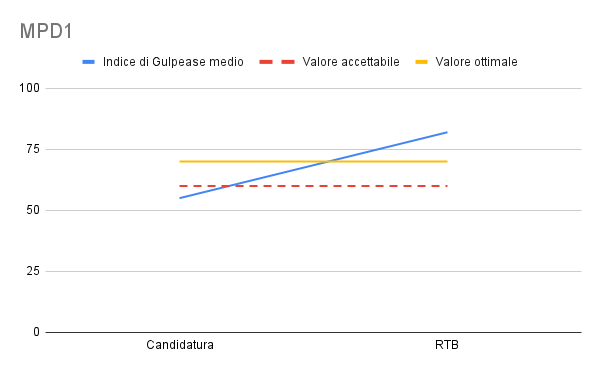
\includegraphics[width=0.7\textwidth]{img/MPD1.png}
    \caption{MPD1 - Indice di Gulpease}
    \label{fig:mpd1}
\end{figure}


\subsection{MPD2 - Copertura dei requisiti}
Non è stato possibile raggiungere il valore ottimale di copertura dei requisiti.\\
Durante la fase PB il gruppo si è reso conto, approfondendo la conoscenza delle tecnologie utilizzate, di aver sottostimato il tempo necessario per l'implementazione delle funzionalità previste all'inizio del progetto.
Questo ha portato ad una ristrutturazione del documento Analisi dei requisiti, riducendo il numero di requisiti obbligatori presenti.
Siccome le ore di lavoro disponibili sono rapidamente state consumate per le attività di codifica, il gruppo ha scelto di non soddisfare parte dei requisiti non obbligatori, preferendo non ritardare la data di consegna del progetto.
\label{s:mpd2}
\begin{table}[H]
    \centering
    \begin{tabularx}{\textwidth}{X|X|l|l|l}
        \hline
        \textbf{Metrica}        & \textbf{Codice} & \textbf{Valore ottimale} & \textbf{Valore accettabile} & \textbf{Valore attuale} \\
        \hline
        Copertura dei requisiti & MPD2            & $100\%$                  & $80\%$                      & $71\%$                \\
        \hline
    \end{tabularx}
\end{table}


\subsection{MPD9 - Browser supportati}
\label{s:mpd9}
Sono stati eseguiti test per verificare il corretto funzionamento dell'applicativo sui seguenti \textit{browser}:
\begin{itemize}
    \item Google Chrome
    \item Arc
    \item Opera GX
    \item Firefox
    \item Safari
    \item Microsfot Edge
\end{itemize}

\begin{table}[H]
    \centering
    \begin{tabularx}{\textwidth}{X|X|l|l|l}
        \hline
        \textbf{Metrica}   & \textbf{Codice} & \textbf{Valore ottimale} & \textbf{Valore accettabile} & \textbf{Valore attuale} \\
        \hline
        Browser supportati & MPD9            & $100\%$                  & $80\%$                      & $100\%$ (6)               \\
        \hline
    \end{tabularx}
\end{table}

\end{document}
